\documentclass{article}
% packages
\usepackage{amsmath,amssymb}
\usepackage{graphicx}
\usepackage{hyperref}

% directory of figures
%\graphicspath{ {figs} }

% latin bold lower
\newcommand{\ba}{\mathbf{a}} 
\newcommand{\bc}{\mathbf{c}} 
\newcommand{\be}{\mathbf{e}} 
\newcommand{\bh}{\mathbf{h}} 
\newcommand{\bp}{\mathbf{p}} 
\newcommand{\bt}{\mathbf{t}} 
\newcommand{\bs}{\mathbf{s}} 
\newcommand{\bu}{\mathbf{u}} 
\newcommand{\bv}{\mathbf{v}} 
\newcommand{\bw}{\mathbf{w}} 
\newcommand{\bx}{\mathbf{x}} 
\newcommand{\by}{\mathbf{y}} 
\newcommand{\bz}{\mathbf{z}} 
\newcommand{\bm}{\mathbf{m}} 

% latin bold upper
\newcommand{\bA}{\mathbf{A}} 
\newcommand{\bB}{\mathbf{B}} 
\newcommand{\bC}{\mathbf{C}} 
\newcommand{\bI}{\mathbf{I}} 
\newcommand{\bJ}{\mathbf{J}} 
\newcommand{\bL}{\mathbf{L}} 
\newcommand{\bM}{\mathbf{M}} 
\newcommand{\bP}{\mathbf{P}}
\newcommand{\bQ}{\mathbf{Q}} 
\newcommand{\bR}{\mathbf{R}} 
\newcommand{\bT}{\mathbf{T}} 
\newcommand{\bU}{\mathbf{U}} 
\newcommand{\bV}{\mathbf{V}} 
\newcommand{\bW}{\mathbf{W}} 
\newcommand{\bX}{\mathbf{X}} 
\newcommand{\bY}{\mathbf{Y}} 
\newcommand{\bZ}{\mathbf{Z}} 

% latin cal upper
\newcommand{\cF}{\mathcal{F}} 
\newcommand{\cG}{\mathcal{G}} 
\newcommand{\cI}{\mathcal{I}} 
\newcommand{\cL}{\mathcal{L}} 
\newcommand{\cM}{\mathcal{M}} 
\newcommand{\cN}{\mathcal{N}} 
\newcommand{\cS}{\mathcal{S}} 
\newcommand{\cT}{\mathcal{T}} 
\newcommand{\cW}{\mathcal{W}} 
\newcommand{\cX}{\mathcal{X}} 
\newcommand{\cZ}{\mathcal{Z}} 

% latin bb upper
\newcommand{\bbE}{\mathbb{E}} 
\newcommand{\bbI}{\mathbb{I}} 
\newcommand{\bbP}{\mathbb{P}} 
\newcommand{\bbR}{\mathbb{R}}
\newcommand{\bbX}{\mathbb{X}} 
\newcommand{\bbY}{\mathbb{Y}}
\newcommand{\bbW}{\mathbb{W}} 

% greek bold lower
\newcommand{\bepsilon}{\boldsymbol{\epsilon}} 
\newcommand{\btheta}{\boldsymbol{\theta}} 
\newcommand{\blambda}{\boldsymbol{\lambda}} 
\newcommand{\bpi}{\boldsymbol{\pi}} 
\newcommand{\bmu}{\boldsymbol{\mu}} 
\newcommand{\bsigma}{\boldsymbol{\sigma}} 
\newcommand{\bphi}{\boldsymbol{\phi}} 

% greek bold upper
\newcommand{\bSigma}{\boldsymbol{\Sigma}} 

\DeclareMathOperator*{\argmin}{arg\,min}
\DeclareMathOperator*{\argmax}{arg\,max}

% transpose
\newcommand{\T}{^{\text{\tiny\sffamily\upshape\mdseries T}}}

% if you need to pass options to natbib, use, e.g.:
\PassOptionsToPackage{numbers, sort, compress}{natbib}
% before loading neurips_2024


% ready for submission
%\usepackage{neurips_2024}


% to compile a preprint version, e.g., for submission to arXiv, add add the
% [preprint] option:
\usepackage[preprint]{neurips_2024}


% to compile a camera-ready version, add the [final] option, e.g.:
%     \usepackage[final]{neurips_2024}


% to avoid loading the natbib package, add option nonatbib:
%    \usepackage[nonatbib]{neurips_2024}


\usepackage[utf8]{inputenc} % allow utf-8 input
\usepackage[T1]{fontenc}    % use 8-bit T1 fonts
\usepackage{hyperref}       % hyperlinks
\usepackage{url}            % simple URL typesetting
\usepackage{booktabs}       % professional-quality tables
\usepackage{amsfonts}       % blackboard math symbols
\usepackage{nicefrac}       % compact symbols for 1/2, etc.
\usepackage{microtype}      % microtypography
\usepackage{xcolor}         % colors

%%%

\usepackage{subcaption}
\usepackage{graphicx}
\usepackage{multirow}
\usepackage{amsmath,amssymb,amsfonts}
\usepackage{amsthm}
\usepackage{mathrsfs}
\usepackage{xcolor}
\usepackage{textcomp}
\usepackage{manyfoot}
\usepackage{booktabs}
\usepackage{algorithm}
\usepackage{algorithmicx}
\usepackage{algpseudocode}
\usepackage{listings}
\usepackage{caption}

\captionsetup[figure]{width=0.7\textwidth}

\newtheorem{theorem}{Theorem} % continuous numbers
%%\newtheorem{theorem}{Theorem}[section] % sectionwise numbers
%% optional argument [theorem] produces theorem numbering sequence instead of independent numbers for Proposition
\newtheorem{proposition}[theorem]{Proposition}% 
\newtheorem{lemma}{Lemma}% 
%%\newtheorem{proposition}{Proposition} % to get separate numbers for theorem and proposition etc.

\newtheorem{example}{Example}
\newtheorem{remark}{Remark}

\newtheorem{definition}{Definition}
\newtheorem{assumption}{Assumption}

%%%


\title{Detecting Manual Alterations in Biological Image Data 
Using Contrastive Learning and Pairwise Image Comparison}


% The \author macro works with any number of authors. There are two commands
% used to separate the names and addresses of multiple authors: \And and \AND.
%
% Using \And between authors leaves it to LaTeX to determine where to break the
% lines. Using \AND forces a line break at that point. So, if LaTeX puts 3 of 4
% authors names on the first line, and the last on the second line, try using
% \AND instead of \And before the third author name.


\author{%
  Georgii Nekhoroshkov\\
  MIPT\\
  Moscow, Russia\\
  \texttt{nekhoroshkov.gs@phystech.edu}\\
  \And
  Daniil Dorin\\
  MIPT\\
  Moscow, Russia\\
  \texttt{dorin.dd.contact@gmail.com}\\
  \And
  Andrii Hraboviy\\
  MIPT\\
  Moscow, Russia\\
  \texttt{grabovoy.av@phystech.edu}\\
}


\begin{document}


\maketitle

\begin{abstract}

    In this paper, we address the problem of detecting manipulations in biological images. 
    Ensuring the integrity of biological 
    image data is essential for reliable scientific research. 
    The study focuses on developing a model for pairwise image comparison
    using contrastive learning, demonstrating high pairwise comparison metrics to detect 
    manual modifications or more subtle alterations. 
    The proposed method outperforms state-of-the-art models, 
    including CLIP and Barlow Twins, in the task of biological 
    image comparison on fMRI scans and cell datasets. 
    This work contributes to automated fraud detection and data validation in 
    biological research.

\end{abstract}

\textbf{Keywords:}
Machine Learning, Pairwise Image Comparison, Self-Supervised Learning, 
Fine-Tuning, Automated Fraud Detection, Detecting Data Alterations

\section{Introduction}\label{sec:intro}

Our work aims to develop a machine learning solution for the problem 
of reusing existing biological and medical snapshots to demonstrate results 
in newly published biological articles. Fake images negatively impact on 
medicine by providing false or fabricated results and undermining the credibility 
of new scientific work in these fields. Existing state-of-the-art self-supervised learning 
approaches demonstrate remarkable results in pairwise image comparison tasks 
(\texttt{SimCLR} \cite{chen2020simclr}, \texttt{CLIP} \cite{radford2021clip}, 
\text{Barlow Twins} \cite{zbontar2021barlow}). 
However, their performance significantly worsens when applied to complex biological data. 
It requires developing model that is more sensitive to subtle changes in the image content 
while remaining resistant to various manual alterations, such as color jittering, 
flipping, rotation, noise application, and random affine transformations. 
At present, the problem of matching biological and medical images remains unsolved due 
to the complexity of distinguishing snapshots of similar objects, where 
differences can only be identified by experts in the field.

We propose a solution, based on \texttt{Barlow Twins} \cite{zbontar2021barlow},
trained and fine-tuned specifically for complex biological scans. 
The model belongs to the family of self-supervised learning (SSL) 
methods, which have been proven to be competitive with supervised representations 
(\cite{chen2020simclr}, \cite{radford2021clip}, \cite{zbontar2021barlow}, \cite{melekhov2016}, 
\cite{grill2020approach_ssl}). By leveraging a pretrained model, 
it does not require large snapshot datasets to achieve state-of-the-art accuracy 
on the \texttt{Haxby fMRI}, \texttt{CIL Epithelial Cell}, 
\texttt{CIL Lymphocyte Cell} datasets. This solution can be widely used by 
biological articles proofreaders to verify the authenticity of provided images and 
detect borrowings from known datasets. 

%\textbf{Contributions.} Our contributions can be summarized as follows:
%\begin{itemize}
%    \item We present...
%    \item We demonstrate the validity of our theoretical results through empirical studies...
%    \item We highlight the implications of our findings for...
%\end{itemize}

%\textbf{Outline.} The rest of the paper is organized as follows...

\section{Problem}\label{sec:problem}

Given dataset $\mathcal{D}$, consisting of $N$ biological snapshots: 

$$ \mathcal{D} = \{d_i \in \mathcal{S}, i \in [0, N)\} $$

where $\mathcal{S}$ is the image space. 

For simplicity, we will refer to a pair of images with the same content 
before alterations as a \textit{similar} pair; otherwise, it will be called \textit{dissimilar}.
Our goal is to build a model $\mathcal{M}$ using self-supervised contrastive learning (SSCL), 
which should be able to distinguish dissimilar pairs of images and identify similar ones. 

Let $x$ and $y$ be two images ($x, y \in \mathcal{S}$).
The model consists of two main parts:

$$ \mathcal{M}(x, y) = h(f_{\theta}(x), f_{\theta}(y))) $$

where $f_{\theta}$ is an encoder with a trainable parameter set $\theta$, and 
$h$ is the linear classifier:

$$ f_{\theta}(x) = v_x \in \mathbb{R}^{d} $$

$$ h(v_x, v_y) = s \in \{0, 1\} $$

Value $s = 1$ corresponds to similar pairs, $s = 0$ represents dissimilar pairs.

%To train the encoder, let us define the loss function $\mathcal{L}$:

%$$ \mathcal{L}(v_x, v_y, I(x, y)) \in [0, +\infty) $$

%where $v_x$ and $v_y$ are the embeddings of images $x$ and $y$, respectively, 
%and $I(x, y)$ is defined as follows:

%$$ I(x, y) = \begin{cases} 
%1, \text{if $x$ and $y$ are similar}, \\
%0, \text{otherwise}
%\end{cases} $$

The model's accuracy will be evaluated by counting the number of correctly classified similar pairs 
and incorrectly classified ones, producing a single accuracy value to compare with other 
state-of-the-art models.

\section{Computational Experiment}

In this section, we conduct an experiment to train the projector of the 
\texttt{Barlow Twins} model on a blood cells dataset. 
Our goal is to determine if the model, with its state-of-the-art pretrained encoder, 
can be successfully adapted to our problem.

The model's encoder is the pretrained \texttt{ResNet50} from the original article
\cite{zbontar2021barlow}. The dataset consists of $320$ images of lymphocyte cells, 
split into a training set of $256$ images and a validation set of $64$ scans. 
The projector is composed of three groups of layers; each group contains a linear layer, 
batch normalization, and a ReLU activation function. 
The input dimensions for the groups are $2048$, $1024$, and $1024$, respectively.

The loss function is identical to that described in the original article. 
For optimization, we use the \texttt{Adam} optimizer with the following learning rate schedule:

$$ q_k = \frac{1}{2} \cdot (1 + \cos(\pi \cdot \frac{k}{K})) $$

$$ \gamma_{k} = \gamma_{start} \cdot q_k + \gamma_{end} \cdot (1 - q_k) $$

where $k$ is the epoch number, $K$ is the total number of epochs, 
$\gamma_{start} = 5 \cdot 10^{-3}$, $\gamma_{end} = 5 \cdot 10^{-4}$. 

\begin{figure}[htbp]
    \centering
    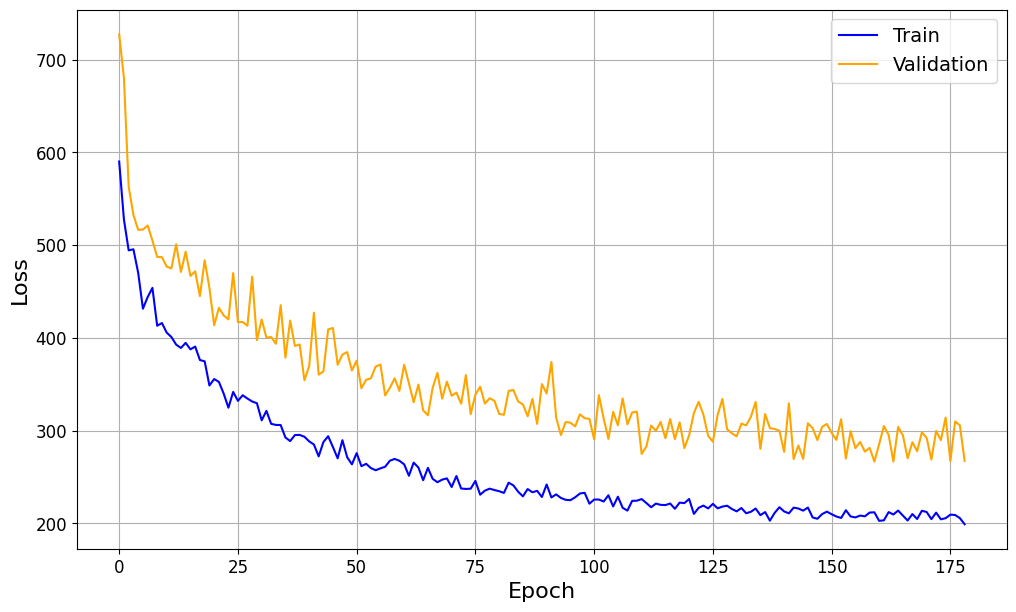
\includegraphics[width=0.95\textwidth]{figures/BT_blood-cells-256_experiment.png}
    \caption{Graph of the loss function for training and validation samples. 
    The experiment was conducted over $180$ epochs. 
    The validation loss decreases alongside the training loss, indicating that 
    the model can be trained further. 
    Training takes approximately $25$ minutes on a Google Colab GPU. 
    }
    \label{fig:experiment}
\end{figure}

\section{Method}

The challenge of detecting reused biological and medical images lies in the difficulty of
distinguishing between visually similar images while maintaining invariance to various 
transformations. Our dataset consists of biological snapshots obtained from publicly available 
sources and is stored as an array $\mathcal{D}$ with elements $d_i \in [0, 256)^{l \times l 
\times 3}$, where $l$ denotes the length of the image sides. We define a \textit{solution} as 
any method intended to address the stated problem, and we refer to the \textit{model} as the 
machine learning solution proposed in our work.

The structure of our model is inspired by the \texttt{Barlow Twins} \cite{zbontar2021barlow}. 
It consists of three deep networks: an embedding function $f$, a projector function $p$, 
and a similarity function $s$ that returns a single number in the range $[0,1]$. 
The embedding network is implemented using a fine-tuned, pretrained \texttt{ResNet50}.

To train the projector, we begin with a batch of images $X$. Each image $x_i$ is 
augmented in two different ways to produce two modified versions, $y_i^A$ and $y_i^B$. 
These two batches of augmented images, $Y^A$ and $Y^B$, are then processed by the 
embedding function $f$ to yield embeddings $E^A$ and $E^B$. The embeddings are subsequently 
passed through the projector function $p$, resulting in the projected embeddings 
$Z^A$ and $Z^B$. These projected embeddings are used to compute the loss function 
$\mathcal{L}$ as proposed in \texttt{Barlow Twins} \cite{zbontar2021barlow}:

$$
\mathcal{L}(Z^A, Z^B) = \sum_i (1 - \mathcal{C}_{ii})^2 + \lambda \sum_{i} \sum_{j \neq i} \mathcal{C}_{ij}^2,
$$

where $\lambda$ is a positive constant, and $\mathcal{C}_{ij}$ is the cross-correlation matrix between the outputs of the two networks along the batch dimension, defined as:

$$
\mathcal{C}_{ij} = \frac{\sum_b z_{b,i}^A z_{b,j}^B}{\sqrt{\sum_b (z_{b,i}^A)^2} \sqrt{\sum_b (z_{b,j}^B)^2}}.
$$

For simplicity, we refer to a pair of images with the same content before augmentation as a 
\textit{similar} pair, and a pair with different content as a \textit{dissimilar} pair. The 
objective of the loss function is to minimize the distance between embeddings of similar pairs 
while maximizing the distance for dissimilar pairs.

For accuracy evaluation, we train the similarity network function $s$ while keeping the 
model's weights frozen. Given a batch of images $X$, we generate two batches, 
$Y^A$ and $Y^B$, where $Y^A$ comprises images from $X$ with random modifications, 
and $Y^B$ is a shuffled version of $X$ with different modifications applied. 
Consequently, for each image $x_i$, there is a corresponding modified image $y_i^A$ 
and a randomly transformed image $y_i^B$, with a probability of $0.3$ that they form a 
\textit{similar} pair. These batches are processed sequentially through the embedding 
function $f$ and the projector $p$, and the resulting embeddings $Z^A$ and $Z^B$ are then 
fed into the similarity function $s$. The function $s$ produces a vector $P$ with values 
in the range $[0,1]$, where each element $P_i$ represents the estimated likelihood that the 
pair $(y_i^A, y_i^B)$ is similar. The similarity network is trained using 
Binary Cross-Entropy (BCE) loss.

The model is trained on $70\%$ of the dataset $\mathcal{D}$, 
validated on an additional $10\%$, and tested on the remaining $20\%$.

\textbf{Topic \#1.}
TODO

\textbf{Topic \#2.}
TODO

\section{Preliminaries}\label{sec:prelim}

\subsection{General notation}

In this section, we introduce the general notation used in the rest of the paper and the basic assumptions. 

\subsection{Assumptions} 

TODO

\section{Experiments}\label{sec:exp}

To verify the theoretical estimates obtained, we conducted a detailed empirical study...

\section{Discussion}\label{sec:disc}

TODO

\section{Conclusion}\label{sec:concl}

TODO


%%%%%%%%%%%%%%%%%%%%%%%%%%%%%%%%%%%%%%%%%%%%%%%%%%%%%%%%%%%%

\bibliographystyle{unsrtnat}
\bibliography{references}

%%%%%%%%%%%%%%%%%%%%%%%%%%%%%%%%%%%%%%%%%%%%%%%%%%%%%%%%%%%%

\newpage
\appendix
\section{Appendix / supplemental material}\label{app}

\subsection{Additional experiments}\label{app:exp}

TODO

\end{document}
